% {
% \usebackgroundtemplate{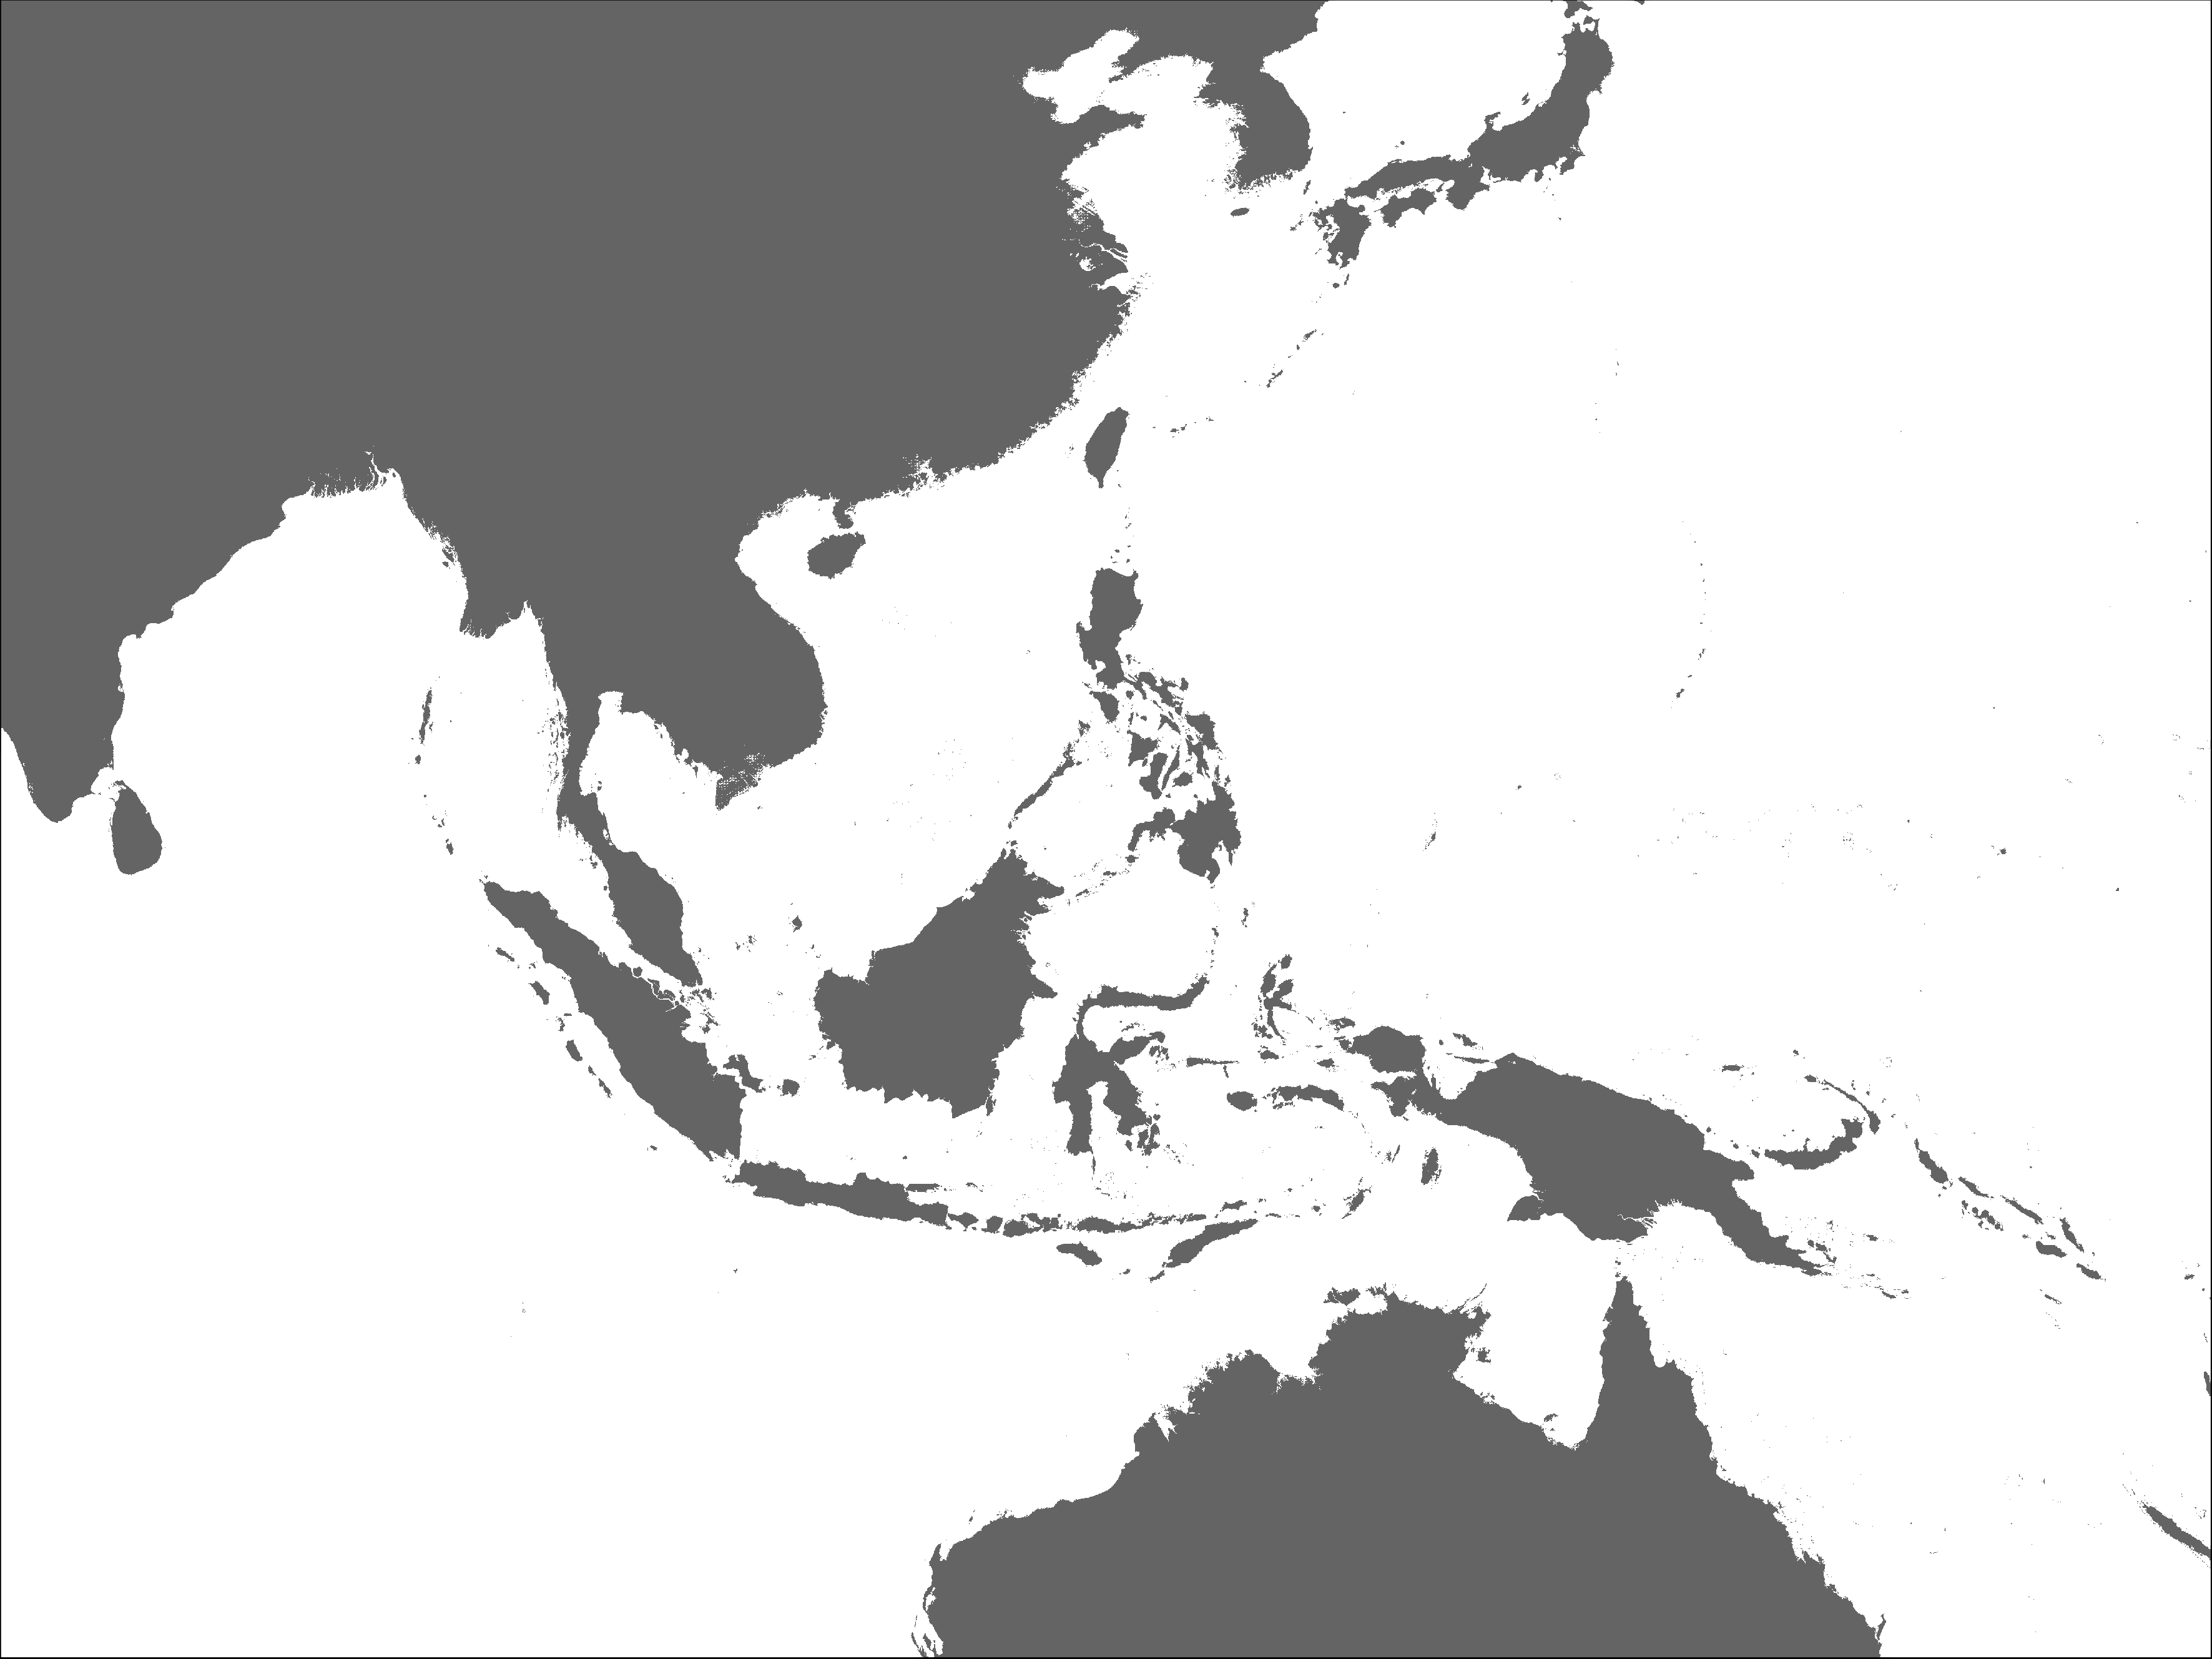
\includegraphics[width=\paperwidth]{../images/maps/se-asia-present.png}}
% \begin{frame}
%     % \frametitle{Climate-driven diversification}    

% \end{frame}
% }

{
\usebackgroundtemplate{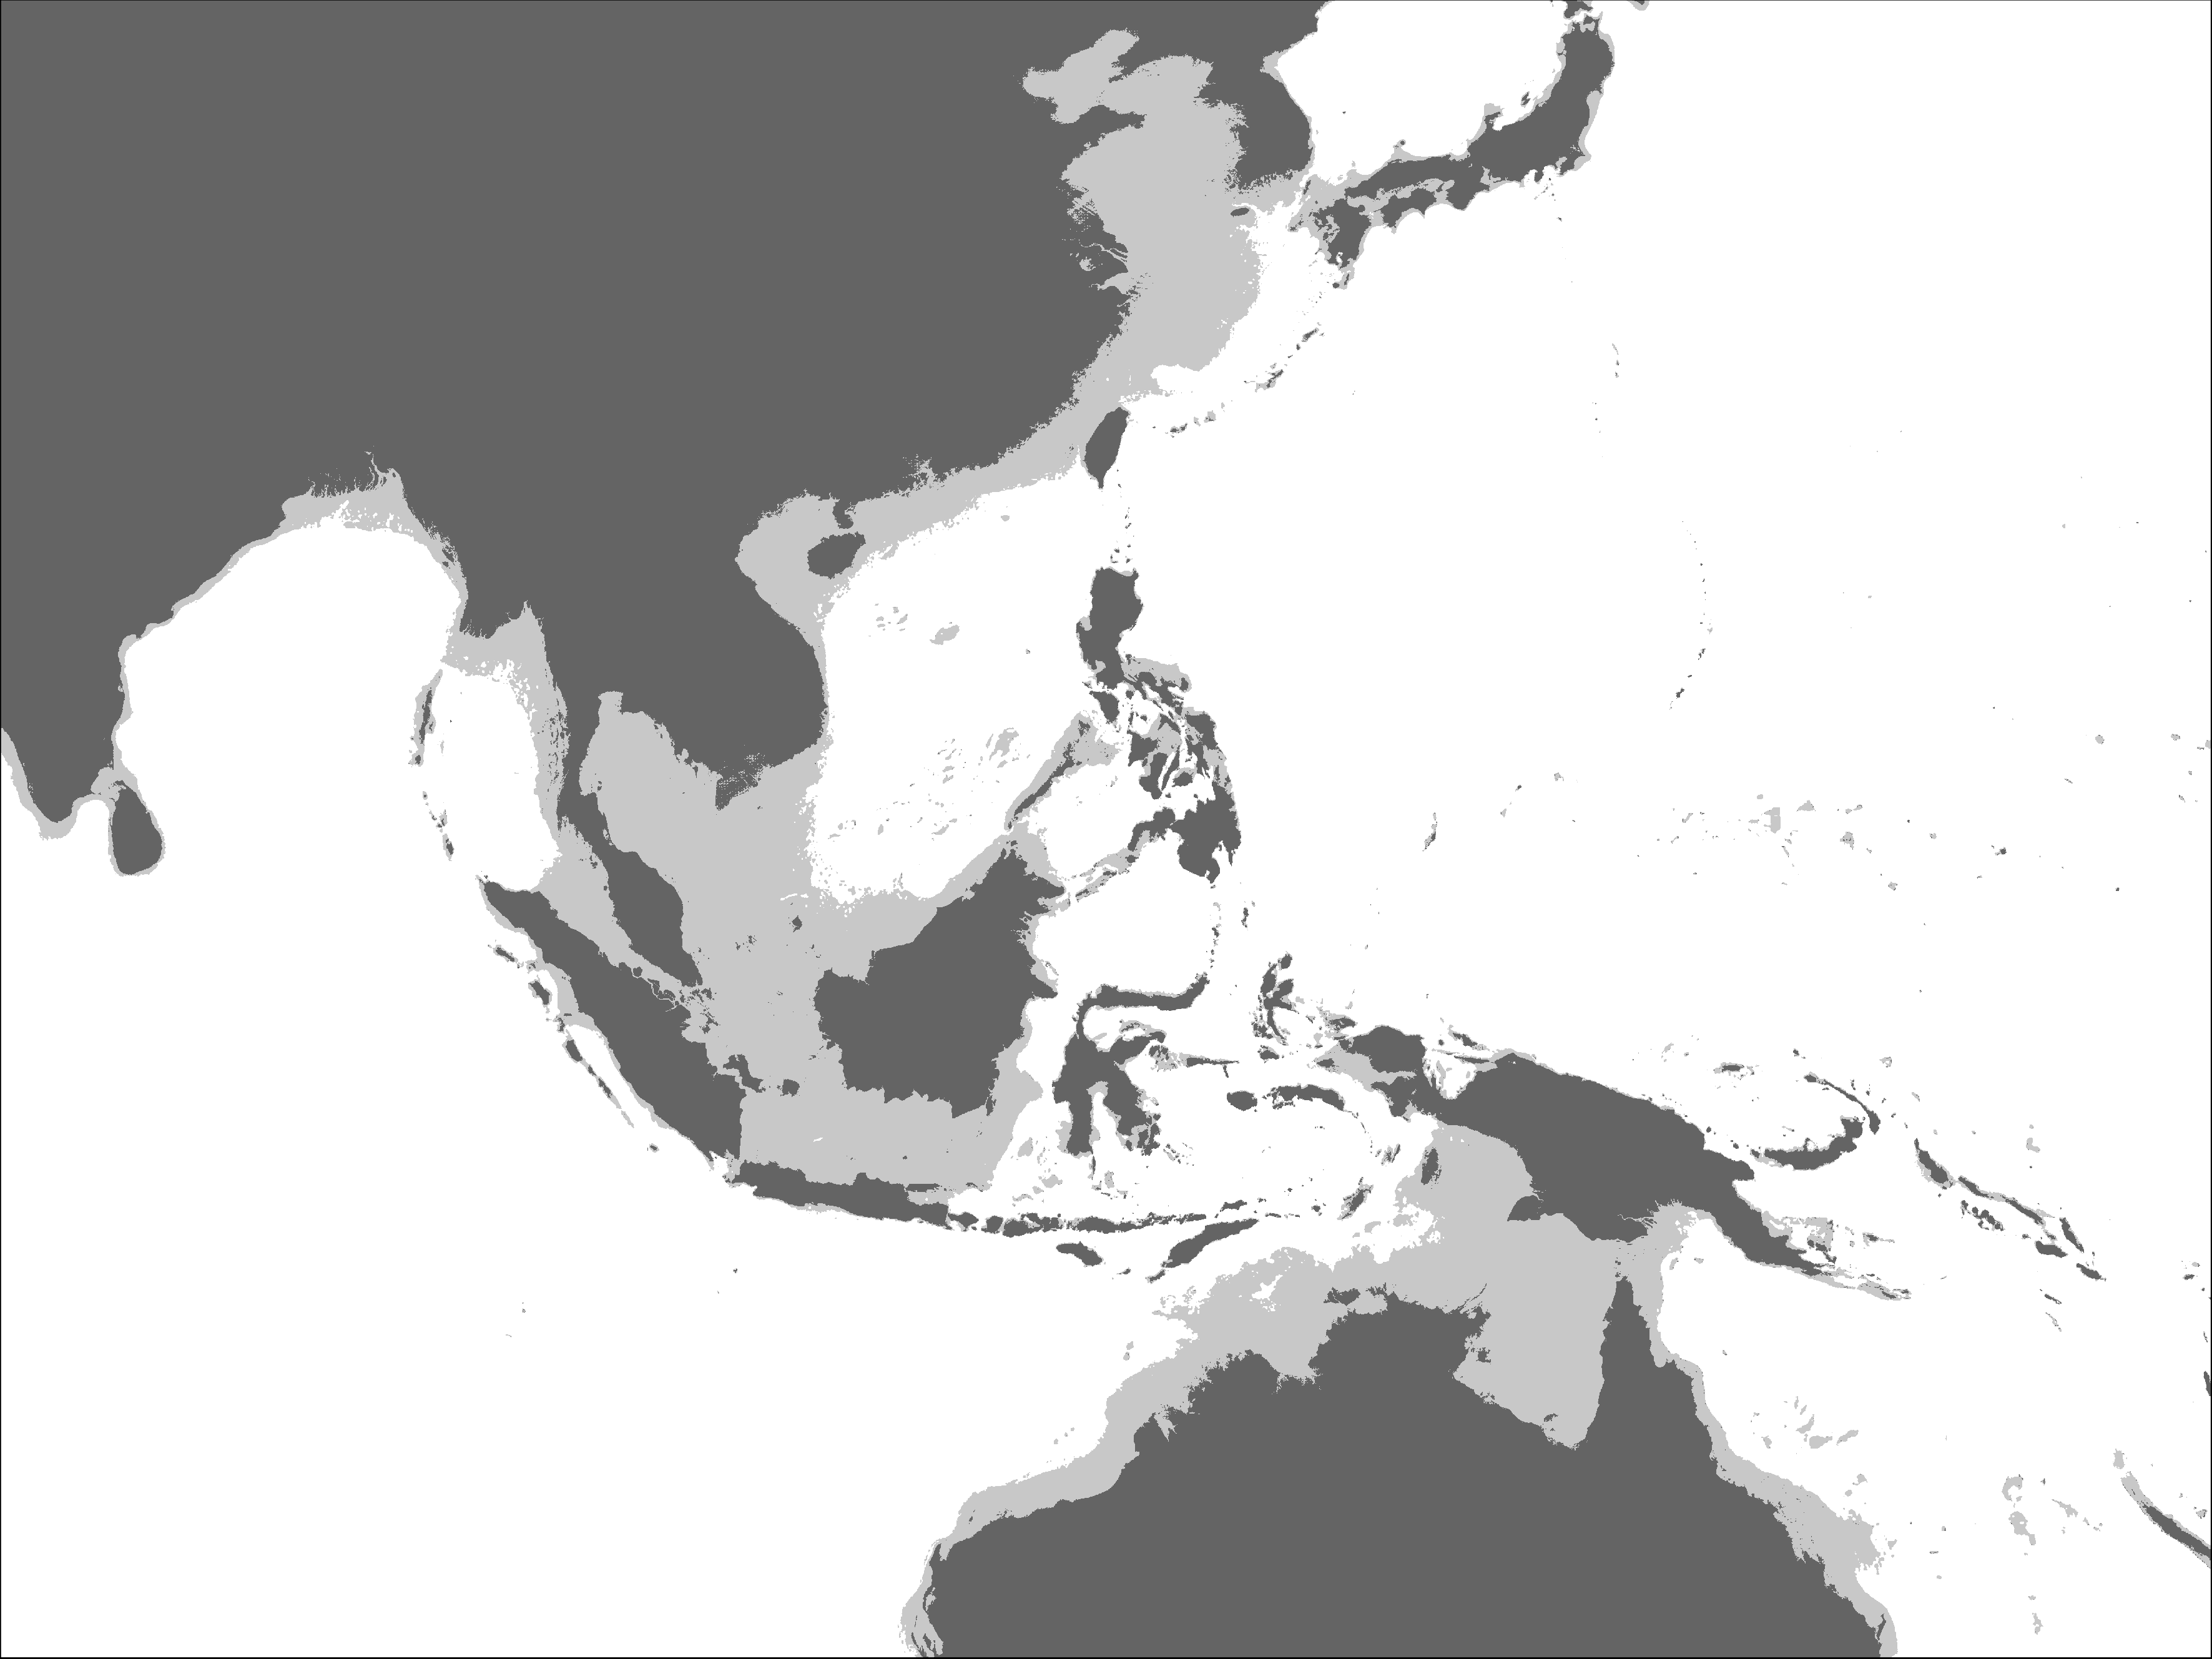
\includegraphics[width=\paperwidth]{../images/maps/se-asia-120.png}}
\begin{frame}
    \frametitle{Empirical application}    
    \begin{columns}
        \column{0.6\textwidth}

        \vspace{6.5cm}

        \ \\

        \column{0.4\textwidth}

        \vspace{-2cm}

        \begin{uncoverenv}<2->
        \colorbox{white}{
            \begin{minipage}[t]{1.0\textwidth}
                \raggedright
                \textbf{Did repeated fragmentation of islands during
                    inter-glacial rises in sea level promote diversification?}
            \end{minipage}
        }
        \end{uncoverenv}
    \end{columns}
\end{frame}
}

\begin{frame}
    \frametitle{Climate-driven diversification}
\begin{columns}[c]
    \column{.5\textwidth}
        \vspace{-1cm}
        \begin{onlyenv}<1>
        \begin{minipage}[t][1.0\textheight][c]{\linewidth}
        \centerline{
        \includegraphics<1>[height=2cm]{/home/jamie/Dropbox/field-photos/people/rafe.jpg}
        \hspace{0.3mm}
        \includegraphics<1>[height=2cm]{/home/jamie/Dropbox/field-photos/people/rob.jpg}}
        \centerline{
        \includegraphics<1>[height=2cm]{/home/jamie/Dropbox/field-photos/people/charles.jpg}
        \hspace{0.3mm}
        \includegraphics<1>[height=2cm]{/home/jamie/Dropbox/field-photos/people/cam.jpg}}
        \centerline{
        \includegraphics<1>[height=2cm]{/home/jamie/Dropbox/field-photos/people/jeet2.jpg}
        \hspace{0.3mm}
        \includegraphics<1>[height=2cm]{/home/jamie/Dropbox/field-photos/people/jake.jpg}}
        \centerline{
        \includegraphics<1>[height=2cm]{/home/jamie/Dropbox/field-photos/people/allie.jpg}
        \hspace{0.3mm}
        \includegraphics<1>[height=2cm]{/home/jamie/Dropbox/field-photos/people/Luke.jpg}
        \hspace{0.3mm}
        \includegraphics<1>[height=2cm]{/home/jamie/Dropbox/field-photos/people/anthony.png}}
        \end{minipage}
        \end{onlyenv}

        \begin{onlyenv}<2->
        \begin{minipage}[t][1.0\textheight][c]{\linewidth}
        \centerline{
        \includegraphics<2->[height=1.3cm]{../images/photos/crocidura-negrina-JAEsselstyn.jpg}
        \hspace{0.3mm}
        \includegraphics<2->[height=1.3cm]{../images/photos/crocidura-beatus-DSBalete.jpg}}
        % \vspace{0.5mm}
        \centerline{
        \includegraphics<2->[height=1.3cm]{../images/photos/hipposideros-obscurus-MRMDuya.jpg}
        \hspace{0.3mm}
        \includegraphics<2->[height=1.3cm]{../images/photos/haplonycteris-fischeri-JHolden.jpg}}
        % \vspace{0.5mm}
        \centerline{
        \includegraphics<2->[height=1.3cm]{../images/photos/sphenomorphus-abdictus-rmb.jpg}
        \hspace{0.3mm}
        \includegraphics<2->[height=1.3cm]{../images/photos/sphenomorphus-arborens-rmb.jpg}}
        % \vspace{0.5mm}
        \centerline{
        \includegraphics<2->[height=1.3cm]{../images/photos/gekko-mindorensis.jpg}
        \hspace{0.3mm}
        \includegraphics<2->[height=1.3cm]{../images/photos/dendrelaphis-pictus-cds.jpg}}
        % \vspace{0.5mm}
        \centerline{
        \includegraphics<2->[height=1.3cm]{../images/photos/cyrt-agusanensis.jpg}
        \hspace{0.3mm}
        \includegraphics<2->[height=1.3cm]{../images/photos/cyrt-annulatus-cds.jpg}}
        % \vspace{0.5mm}
        \centerline{
        \includegraphics<2->[height=1.3cm]{../images/photos/limnonectes-magnus-cds.jpg}
        \hspace{0.3mm}
        \includegraphics<2->[height=1.3cm]{../images/photos/limnonectes-leytensis-rmb.jpg}}
        \end{minipage}
        \end{onlyenv}

    \column{.5\textwidth}
        \vspace{-1cm}
        \begin{minipage}[t][1.0\textheight][c]{\linewidth}
        \includegraphics<1-2>[width=\textwidth]{../images/maps/Philippines.png}
        \includegraphics<3>[width=\textwidth]{../images/maps/Philippines-negros_panay.png}
        % \begin{onlyenv}<4->
        %     \begin{itemize}
        %         \item Strong support for simultaneous divergence of all 22 taxon pairs
                
        %         \item Posterior probability $>$ 0.96 \\
            
        %         \item $\sim$100,000--250,000 years ago
        %     \end{itemize}
        % \end{onlyenv}
        \end{minipage}
\end{columns}
\end{frame}

\begin{frame}
    \frametitle{Results}
    \begin{adjustwidth}{-4.5em}{-2.5em}
    \begin{columns}
        \column{0.3\linewidth}
    \begin{itemize}
            \small
        \item<2-> Results consistent with prediction of clustered
            divergences
        \item<3-> Results suggest multiple interglacial periods were important
            drivers of diversification and community assembly across Islands of
            Southeast Asia
        \item<4-> However, there is a lot of uncertainty!
    \end{itemize}
        \column{0.6\linewidth}
    \centerline{
    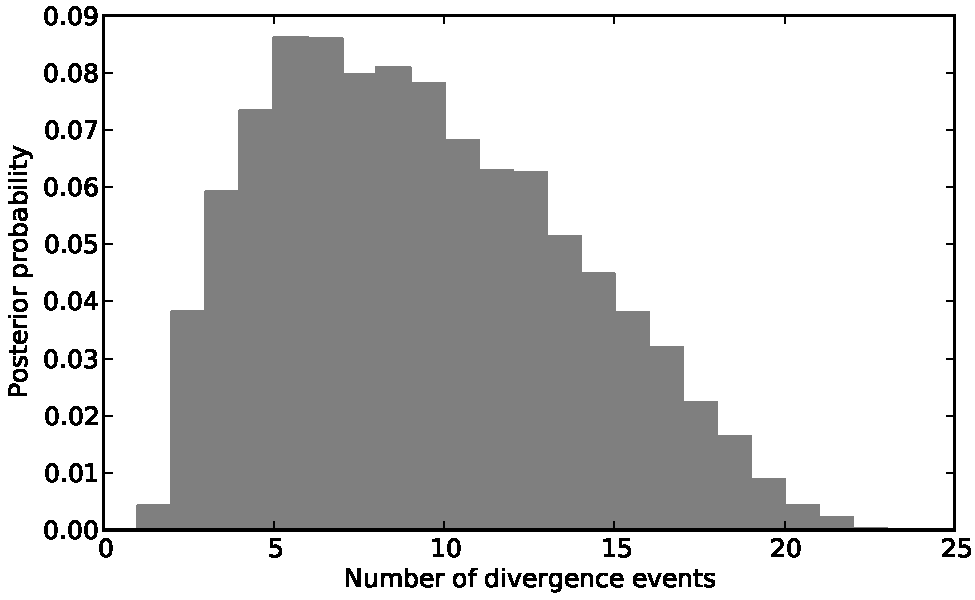
\includegraphics[width=0.85\textwidth]{../../empirical-analyses/plots/philippines-dpp-psi-posterior.pdf}}
    \smallskip
    \centerline{
    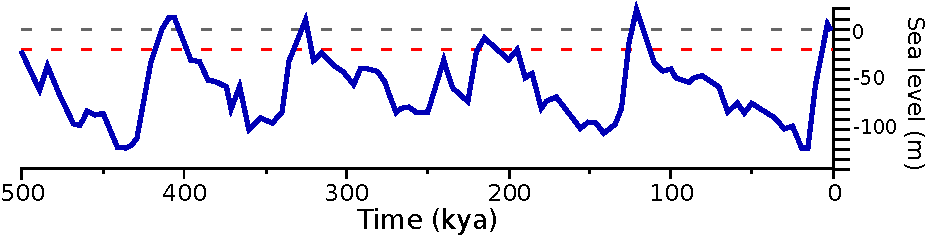
\includegraphics[width=0.8\textwidth]{../images/sea-level-only.pdf}}
    \end{columns}
    \end{adjustwidth}
    \barefootnote{\shortfullcite{Oaks2014dpp}}
\end{frame}

% \begin{frame}
%     \frametitle{Results}
%     \begin{itemize}
%         % \item \textbf{dpp-msbayes allows biologists to leverage comparative
%         %         genomic data to assess the affects of community-scale processes
%         %         on biodiversity}
%         \item<1-> Results consistent with prediction of clustered
%             divergences
%         \item<2-> Results suggest multiple interglacial periods were important
%             drivers of diversification and community assembly across Islands of
%             Southeast Asia
%         \item<3-> However, there is a lot of uncertainty!
%     \end{itemize}
%     \barefootnote{\shortfullcite{Oaks2014dpp}}
% \end{frame}

